
\chapter{Implementation}
This chapter coverages what was done to the Päikky system in order to get it working also during the Internet connection shortages, and how that was done. 

This chapter is concerned with the facts of what the offline mode consists of and how it was implemented. Reasoning for the decisions made are also explained. Analyzing the consequences of those decisions are done later on Chapter~\ref{chap:evaluation}.

%% --------------
\section{The Goal for the Offline Support}
% tämä case päikky -lukuun?

% Mitä Offline-modella TAI SIIS SUPPORTILLA pyrittiin saavuttamaan?
% <META: Pitäisikö yleisemminkin erottaa offline TUKI ja kindergarten-UI:n offline MOODI? Tulisiko tämän tavaran olla jossain muualla kappaleessa kuin täällä?>

The primary goal for the offline support on Päikky was to enable the most critical tasks for kindergarten nurses on all situations on the Kindergarten UI (the mobile friendly version of the Päikky system). 

Päikky's main and the most important feature is the ability to track the attendance of the kindergarten's children on real time. In order to achieve that, nurses must be able to mark the children's coming and going without getting interrupted by the limitations of the application. In order to offer offline support on the Kindergarten UI, a new feature called \textit{Offline mode} was implemented. Offline mode aims at removing the Internet connection quality related limitations on the nurses' key activity. Nurses should be able to use the children logging feature on Päikky under any kind of Internet condition. If the Internet connection is nonexistent, the application should record user's actions and save them to the server once the Internet connection is achieved again.

The secondary goal for the offline support were to allow as seamless usage as possible of the Päikky on kindergartens where Internet connection is weak. Nurses should be able to see the information from Päikky even if there is no Internet connection at the time. Information should be served based on the best-effort delivery: application should show all the information it has at the time to the user while trying to fetch the most latest version of the information.

Other parts of Päikky, the \textit{Manager UI} and the \textit{Family UI}, were left out of the offline support.

The ultimate vision -- yet to be reached -- for the offline support is that it would abstract the Internet connection quality completely away from the user's consideration. Under any connection quality the user should be able to use Päikky normally without any interference. In the current version this is not yet achieved (nor was it scoped to be achieved). % saisko tähän kappaleeseen jonkin viitteen johonkin käytettävyys-diibadaapaan, johonkin käyttäjän "mielenmalleihin" tms eli siis että ultimate goali olisi, ettei käyttäjän tarvitsisi huolehtia tuosta verkon laadusta ollenkaan, jopa niin että käyttäjä ei edes tietäisi ollaanko online- vai offline-moodissa?




%% --------------
\section{State Transitions to and from the Offline Mode}
% offline ja online -moodin selitykset, termien avaus? erityisesti "online-moodi" (jos online-moodia ei selitetä, niin sitten ainakin pitää muissa kappaleissa puhua jostain muusta kuin online-moodista)

% HOX onko päällekkäisyyttä methods-case -kuvauksen kanssa?
Implementation of the offline support to the Kindergarten UI made it to have two different states related to the Internet connection status. Application is on the already mentioned \textit{Offline mode} when the Internet connection is poor or nonexistent, and on the \textit{Online mode} when the Internet connection is working normally. 

The current mode is implicated to the user clearly: while in Offline mode, the Kindergarten UI's header changes color scheme to greyscale and the title says directly \textit{"You are working on the offline mode"}, localized to the user's language.

While in Online mode the Kindergarten UI works almost identically as it did before the offline support implementation. Major changes are that all the API requests done to the Päikky backend are cached to the Local Storage of the device running the Kindergarten UI. Also the sending of Presence marking changes to the backend are done by a dedicated component. Both of these are primarily refactoring the inner parts of the Kindergarten UI, while using the application the user should not experience any difference to the versions prior from these changes.

When entering the Offline mode the method on how data is fetched changes. Instead of fetching the data user requests from the backend, the Kindergarten UI fall backs to the data cached on the \textit{Local Storage}. This will not guarantee the availability of the up-to-date information to the user, but at least showing the best effort version is possible. Due to the nature of the Päikky's data, in most of the cases this is acceptable (for example when looking for children's parents' phone numbers, and other similar data that is not altered on daily basis). Also some of the features on the Kindergarten UI are disabled when the Offline mode comes active. %This functionality is described thoroughly on the Section~\ref{subsec:localstorage}.

While the Offline mode is active, the component responsible for sending the Presence marking changes -- the \textit{Job Queue} -- also acts differently. If there is a recognized issue with the Internet connectivity (which triggers the Offline mode to be activated), Job Queue stops sending the Presence Markings to the backend but instead saves them to the Local Storage. User is notified on this by showing all the time the size of the queue on the top right corner of the Kindergarten UI. When the Internet connection is active again, the Job Queue starts to send the cached Presence Markings to the backend one at a time. %This functionality is explained in depth on the Section~\ref{subsec:jobqueue}.





%% --------------
\section{Limited Feature Set in Offline Mode}
\label{sec:limitedfeatureset}
% Offline-moden rajoitettu featuresetti - mitä ja miksi

Similarly to many other real life software project, also in Päikky compromises have been made while balancing between the scope, available resources, and the quality of the end product. In order to create software with good quality under given budget, the scope had to be kept reasonable and some prioritization between features had to be made. This resulted the first version (the one studied by this thesis) to be technically quite simple and even naive on some aspects. Users experience this as a lack or disabling of some features on the offline mode.




%% ###
\subsection{Disabled Features}
When the application enters the Offline mode all the features except the critical key functionality are disabled from the user. These include features such as

\begin{enumerate}
    \item sending messages in the application,
    \item editing persons' information,
    \item changing persons' photos,
    \item editing existing \textit{presence markings} or upcoming \textit{presence plans}.
\end{enumerate}

These features were left out from the Offline support based on feature importance evaluation done by the client organization. % REMOVED BY TOMMI'S REQUEST [Since under available budget some features had to excluded from the offline mode, the ones listed above were selected due to the nature of their basic use case.]

None of the listed activities are essential for the Päikky's key feature, the real time tracking of kindergarten's personnel attendance. If there is no Internet connection available at the time, each one of these activities can be postponed without sacrificing the integrity of the presence data on the system until the Internet connection is available again.




%% ###
\subsection{Simplified Data Synchronizing}
% synkkaus-yksinkertaistus-juttui
% nonexistent collision check!
% googlewavepaprusta jotain dadaaa tänne?
The nature of the Päikky usage by the nurses allowed the development team to make some simplifications to the implementation of the offline mode. These simplifications included the way how conflicts between concurrent changes are solved. To put it bluntly, they are not solved in any way.

To understand why this solution was feasible, one has to understand the environment and practices about how Päikky is operated. The usual scenario in  kindergartens where Päikky is used is that each kindergarten group has only one dedicated device. With minor exceptions all of the presence markings for the care group's personnel are done via the group's dedicated device, which is also the only device for the group to access Päikky. This is also the way how usage of Päikky is instructed by the client organization to the kindergarten personnel. Editing person's presence status from different devices while on offline mode is especially discouraged. With these guidelines the probability for cases where two different devices have made concurrent changes to individual person becomes almost non-existent. 

These circumstances allowed the development team to streamline the data synchronization on the Päikky server. On agreement with the client organization, there is no functionality that tries to solve possible merge conflicts on the presence data. If there appears a situation where two devices have concurrently changed the attendance status of a single person -- contrary on the instructions given to the users -- both of the changes are saved to the database. Fixing the data to reflect the situation happened in the real world is left to the responsibility of the kindergarten personnel.

The decision which passed on the responsibility of the data correctness to users also removed functionality needed on the Päikky backend. Because of this the work done in order to implement the required level of offline support to Päikky was almost entirely done to the Kindergarten UI. The backend required only minimal changes relating this. The backend changes that were required are explained in depth in Subsection~\ref{subsec:backend-implementation}. 

The decision of implementing no merge conflict solving strategy removes the need of offline related functionality on the Päikky server almost completely. By this the development effort was cut significantly: the probability of creating data conflicts has been made minimal with the user instructions, and in the implausible case of a conflict to appear resolving it is left to the responsibility of the user, not by the code base. 

From the server point of view, presence markings done on the offline mode are received and stored exactly same way as are the markings done real time on the online mode. Only thing that differs is the time gap between the presence marking's timestamp and the occasion when the presence marking is received on the server. 





%% ----------------------------------
\section{Technical Details}
% HOX tää koko setti on lähinnä frontendissä, backendiin ei juurikaan tehty mitään lisätemppuja offline-moodia varten??
The technical details of the implementation cover almost entirely only the Kindergarten UI of the Päikky system. This is due to the allowed boundaries for the development team and the real life limitations of the Päikky system usage. In order to achieve the required level of offline support on the system, almost all of the work could have been done only on the mobile frontend codebase: the Kindergarten UI. In addition to the changes made to the backend, no other modules (\textit{Family UI, Manager UI}) of the system needed changes. However the other modules did not gain any kind of added offline support either.


%% ###
\subsection{HTTP Cache Headers}
\label{subsec:cacheheaders}
% maininta, että tämä olisi ollut hyvä tehdä myös ilman offline-tuen tekemistä
% IMPR:
% - pitäisikö tänne vielä erotella API-pyynnöt omiksi jutuikseen? Nehän tulee tosin Tomcatilta, käpisteleekö Apache sinne headereita ollenkaan? 
% -> API-pyynnön response headerit:
% Access-Control-Allow-Origin:*
% Connection:Keep-Alive
% Content-Type:application/json;charset=UTF-8
% Date:Mon, 24 Nov 2014 12:45:59 GMT
% Keep-Alive:timeout=5, max=99
% Server:Apache-Coyote/1.1
% Transfer-Encoding:chunked

% mahdollisia viitteitä:
% - http://tools.ietf.org/html/rfc2965 (????)
% - http://www.w3.org/Protocols/rfc2616/rfc2616-sec14.html#sec14.9 !

Starting point for the offline support implementation was to take as much advantage as possible from the techniques already in use on the Päikky system's implementation. The first task for the development team was to ensure that the cache related features of the HTTP protocol were utilized thoroughly.

Previously there were issues reported by the users after production environment updates that the new features announced were not visible on their devices. This was the result of poor and some part nonexistent cache header usage. The cache headers prior the change instructed the browser to save the \textit{index.html} document -- the starting point of the Kindergarten UI web application -- and all the JavaScript files for 24 hours on the file system of the device. If those files were requested within that 24 hours, the cached versions were used. This created a huge lag on the rollout of the latest version to the end users' devices, which caused work for the development team since both the old and the new version of the frontend client had to be supported on the backend.
% HOX tsekkaa tästä kappaleesta toi vanhan cachetusajan pituus, emmä muista, tuo 24h on vejetty stetsonista :----D 

The ``release lag'' was addressed by altering the HTTP 1.1 headers related to caching, which are returned by the Päikky backend's Apache web server to the browser. The first solution was to disable cache entirely, forcing the browser to fetch the data again each time from the backend while browsing. This was achieved via headers described in Listing~\ref{lst:cacheheader-1}.

% päikky main.js -nykyrequsta:
\begin{lstlisting}[caption={Päikky HTTP Cache Headers},label={lst:cacheheader-1}]
    Cache-Control:max-age=0, no-cache, no-store, must-revalidate
    Pragma:no-cache
    Date:Mon, 24 Nov 2014 08:36:04 GMT
    Expires:Wed, 11 Jan 1984 05:00:00 GMT
\end{lstlisting}

The goal with these headers is that the browser saves intentionally none of the content it receives. Achieving this is done by several mechanisms to cover the most of the browsers in use. From the HTTP 1.1 protocol view of point some of the instructions overlap each other (for example \texttt{Pragma:no-cache} and \texttt{Cache-Control:no-cache}) while some are there to address the HTTP 1.0 protocol (using \texttt{Expire-date} from the past). \cite{fielding_et_al_hypertext_????}

Using these headers solved the release lag problem and streamlined the production deploy process, but otherwise did little to actually help the development team to get closer to the offline support on the system. Actually these changes made the Kindergarten UI to be more reliable on Internet connection, since browsers were instructed not to save any data fetched from the Päikky backend. This also increased the average loads of the backend.

To take advantage of the HTTP Cache Headers from the offline support perspective, different cache rules were made for the most bandwidth-greedy assets: the images. On the backend, the following headers were set to be sent on response to each request that were made for images, no matter if they were graphical assets to the web application (icons etc) or profile pictures of children and nurses:

% päikky kuva-nykyrequsta:
% (86400s == 24h)
\begin{lstlisting}[caption=Päikky HTTP Cache Headers for images]
    Cache-Control:max-age=86400
    Content-Type:image/jpeg
    Date:Mon, 24 Nov 2014 12:41:01 GMT
    Expires:Tue, 25 Nov 2014 12:41:01 GMT
\end{lstlisting}

These headers allow the browser to cache the image for 24 hours. For person profile pictures there will not be any lag on updates when the image changes. Every picture gets a generated unique file name on the upload, so from the browser's point of view they are totally new pictures instead of new version of the old picture. The cache validness duration can therefore be decided based only on how fast the update cycle on the graphical assets of the needs to be. If generating unique names for the graphical assets would be done on the production version build phase, this cache duration could be increased to for example one year and only side effect would be increased cache sizes on the clients' browsers.

Addressing the HTTP cache header related problems were not directly coupled to the enabling of the offline mode, but fixing them would have benefit the Päikky system even if the offline support would not have been on the product's road map.







%% ###
\subsection{Application Cache}
\label{subsec:appcache}
% Tänne kappaleeseen saa tarvittaessa paljon lisää kamaa tosta "appcache is a douchebag" -artikkelista, sudenkuoppia jne
% responsiiviset erilaiset kuvat -issuesta maininta?

% UHHHH TIMANTTISTA LÄHDETTÄ TÄÄLLÄ http://dl.acm.org/citation.cfm?id=2307649 katso erityisesti kohta "[3]" !!! [Qian et al.]

HTML 5 specification adds a new tool aiding the creation of offline supported web applications: the Application Cache. The specification was designed to allow creating of web applications that would work (after caching) without Internet connection, but it is also useful in decreasing load and start up times in a normal, Internet-aided usage. \cite{wharry_html5_2014}

Application cache is initialized by creating a Cache Manifest file for each HTML document. In Single-Page Applications, which Päikky also is, this is achieved easily since as the name implies there is only a single HTTP document for the whole web application that needs to be loaded \cite{_html_????}.  Whereas HTTP headers regarding cache rules addresses the problem with generic information about the expiry date of the fetched resources, cache manifest states more elaborate instructions for situations where Internet connection is unavailable. \cite{qian_web_2012}

\newpage

\begin{lstlisting}[caption={Snippet of Päikky's Cache Manifest},label={lst:manifest}]
    CACHE:
    js/configurations/local.js
    js/main-b13f3e6.js
    img/icon_delete.png
    img/paikky_logo.png
    css/client.css

    NETWORK:
    *
\end{lstlisting} % Snippet from the Päikky Kindergarten UI's Application Cache Manifest

In Listing~\ref{lst:manifest} a shortened version of the Cache Manifest of Päikky's \textit{index.html} can be seen. The manifest describes the nature of the applications resources regarding network status to the browser. On the complete version of the Päikky's manifest each of the known resources for the application is listed under the \texttt{``CACHE:''} notation, which means that these resources should be cached by the browser. After that everything else is whitelisted with the \texttt{``*''} wild card to be downloaded from the network. The whitelisting of the rest of the possible resources is important, since when working with the Cache Manifest browser tries to do exactly as stated on the manifest. This means that if that wild card network rule would be removed, the browser would not be able to fetch the resources not listed on explicitly stated on the manifest. \cite[page 212]{lawson_introducing_2011}% hox tuosta serverin lataustavasta ei ole mainintaa tuossa kirjassa (ainakaan en löytänyt vielä), vaan se on peräisin appcache-douchebag-artikkelista

% REDUNDANTTIA TAVARAA 
%The Application Cache also differs from the HTTP caching by not defining expiration dates for individual resource, but instead all of the cached resources are re-downloaded every time when the manifest updates. If the expiration date set to the resource concurs before updating of the manifest file, the resource is re-downloaded. Also when using the 

When using the Cache Manifest, it must be noted that even when the user is online, the files are served from the Application Cache. Developers must also notice that updating the resources listed on the Cache Manifest is not enough. The browser does not re-download them if the manifest itself is not updated (or if the cache expiry date set by the HTTP headers for individual resource does not expire). When visiting a site with a cache manifest again, the browser renders the first version of the site with resources stored on the Application Cache, and only after that connects to Internet for checking possible updates to the content. \cite{archibald_application_2012}

Due to the nature of the cache manifest (has to be updated on every web application update, has to handle each of the resources somehow) it is highly recommended that the creation of the manifest file is automated as a part of the build process of the web application. In Päikky's Kindergarten UI, this is done with the \textit{grunt-manifest} tool every time a new production version is created. For the development environments, a different, static cache manifest is used, which tells the browser not to use the application cache at all.

It is also possible to insert a fallback version for the resources on the Cache Manifest that are used if the network connection is unavailable. In practice the manifest can state alternate version for resources to be used, if there is no network connectivity. This can be useful in some browser heavy applications that use minimal amount of data from the Internet, for example applications like \textit{Google Spreadsheet}\footnote{http://spreadsheet.google.com/} \cite{_using_????}. However this was not seen useful on the implementation of Päikky's offline support and therefore was not used. 

As was the case with the HTTP Cache Headers, the Cache Manifest would also have benefit Päikky even if the offline support would not have been implemented to the system.

% pitäisikö täällä mainita jotain tästä http://alistapart.com/article/application-cache-is-a-douchebag ?






%% ###
\subsection{Monitoring Connection Quality}
\label{subsec:connection-monitoring}
Identifying connection issues is a key activity regarding the Offline mode. When a connection issue is noticed, the Kindergarten UI fall backs from the Online mode to the Offline mode. While on the Offline mode, the application must monitor the health of the connection to determine when it is safe to use the network connection again.

On Päikky the connection quality is monitored via errors on \textit{Ajax requests} \cite{_.ajaxerror_????}, triggered by the \textit{jQuery}-library. As described before, the Kindergarten UI communicates to the backend via REST API requests for different kind of resources. There is an application level error handler for cases when one of these requests should fail. Main part of this handler can be seen in Listing~\ref{lst:offlinetrigger}.

\begin{lstlisting}[caption={Code Snippet which triggers Päikky's Offline Mode},label={lst:offlinetrigger}]
    // Function for identifying network related Ajax errors
    var isOfflineTriggerError = function(thrownError) {
        return _.contains([
            'timeout', // "JavaScript-level" timeout
            ''         // "network-level" errors - all of them
        ], thrownError);
    };

    // Error handler for Ajax errors
    $(document).on("ajaxError",
        function (e, jqXHR, ajaxSettings, thrownError) {
        // List of exceptions that triggers offline-mode
        if (networkStatus.isOfflineTriggerError(thrownError)) {
            vent.trigger('offline');
        }
    });
\end{lstlisting}

In practice Kindergarten UI triggers Offline mode on two different kind of errors: if there is a error coming from the JavaScript-level (usually meaning that no response for request was received within the configured time period) or if there was an error on the network level (connectivity was nonexistent). In these cases, an \textit{offline-event} is triggered via the \textit{vent}, the event bus of the application.

Modern browsers also implement the \textit{navigator.onLine} property, which indicates the network status as a boolean value. Despite the promising specification this can not be the only way of checking the network connectivity, since the behaviour is heavily dependent on the browser. For example in \textit{Chrome} and \textit{Safari} having only a connectivity to local area network will result the \textit{onLine} property being true. \cite{_window.navigator.online_????}

After the application has entered the Offline mode, it halts all the Ajax requests except a specified \textit{ping}-request to the backend which is used to determine the health of the connection. If the ping should fail, another ping request is scheduled. There is a maximum time interval configured on the application in which the response must be received. Only after a successful ping request within the allowed time range the pinging is stopped and the Online mode is activated again.

% tänne vois kirjottaa pingin yhteydessä tapahtuvasta kellosynkkauksesta, jos tarvii lisätekstiä? muuten ei ehkä hirmu oleellinen network statuksen suhteen
% iteasiassa onko sittenkin, sitähän käytetään noiden presence markingien teon yhteydessä




%% ###
\subsection{Using Local Storage as a Cache}
\label{subsec:localstorage}
% Local storagen perusteet
% REST-API-pyyntöjen cachettamisesta local storageen juttua
% hox [Casario et al]

The new HTML5 standard adds also another important tool for the Päikky's offline support to take benefit from: the \textit{Local Storage} \cite{w3.org_web_????}. It is an origin specific storage which saves its contents to the user's file system and persists them between sessions. While being only a simple key-value -storage it is not the most sophisticated solution for client-side storage mechanisms there is available on the modern web development toolbox, but for simple use cases like the Kindergarten UI its simplicity is a decisive advantage.

While being on the Online mode, every request made by Kindergarten UI to the backend's API is stored to the Local Storage. The request's URL is used as the key for the entry, and the response of request is saved as a value for that key. At the current version of the application there are no optimization mechanisms implemented with the Local Storage content. When Internet connection is available the saved responses are ignored. On each request, the possibly already existing responses are overwritten.

After the Offline mode is activated the Kindergarten UI continues to make API requests based on user's actions. But instead of making them to the backend's API, the \textit{Backbone}-library -- which is responsible for data fetching and synchronizing on the application -- forwards the requests to the Local Storage API, where cached versions of the once fetched requests can be found. This allows the user to navigate within the application and see the latest version he/she has fetched from the backend. If the user navigates to a view not visited before, view without the actual content is rendered. 

Due to the limited feature set of the Offline mode there is no need for checking dirty cache entries \cite[page 138]{laplante_dictionary_2000}, since user can not alter the cached data while having no Internet connectivity. Only after the Online mode is activated the editing of the data is made possible, and then the contents of the cache is ignored. Exception to this are the \textit{Presence Markings}, whose are explained in more detail on the following section.


% miksi tämä tehdään local storagella eikä esm cache manifestilla? -> selitä(?

% HOX tietoturvaongelmat tämän suhteen (ei tässä keississä mutta yleisesti), problematiikka tämän tiedon kryptaamisesta -> ei mahdollista







%% ###
\subsection{Job Queue: Promise-based Presence Marking Queue}
\label{subsec:jobqueue}
% Kuuluiskohan tuo promise-konseptiosa related researchiin ennemmin?
% hox presence markingien LUONTI vs. olemassaolevien muokkaus?

% https://github.com/futurice/mukavait-paivahoito-kindergarten-ui/blob/development/src/js/JobQueue.js

The key activity for nurses recognized before on this thesis is the altering of the kindergarten's personnel presence data. This activity must be available for user no matter what the Internet connection status is. Allowing this activity was also the primary goal for the offline support to have. With the resource limitations the development process had it was therefore apposite to create a dedicated mechanism for syncing specifically this data and disabling other data altering features while the Offline mode is active. % IMPR-hox oliko näin?:-D

In the Kindergarten UI, this is enabled by a component called the \textit{Job Queue.} Job Queue is an array of jQuery's \textit{Promise} objects. Each objects in the array represents a single Presence Marking to be saved to the backend. Every time the user creates a new Presence Marking, it is added to the queue, no matter if there is an Internet connection problem recognized or not.

% HUOM .promise jquery specistä:
% The deferred.promise() method allows an asynchronous function to prevent other code from interfering with the progress or status of its internal request. The Promise exposes only the Deferred methods needed to attach additional handlers or determine the state (then, done, fail, always, pipe, progress, and state), but not ones that change the state (resolve, reject, notify, resolveWith, rejectWith, and notifyWith).

The concept of "promise" was first time introduced in 1976 by Friedman and Wise \cite{friedman_impact_1976}. It is used to describe an object whose value is yet to be resolved, being a temporary placeholder and a \textit{promise} for the to-be value. In asynchronous languages such as JavaScript this is highly useful since for example when fetching data the developer can not trust that the results are available immediately after the request. Promise makes sure that altering the state or the progress of its internal request is not possible from outside. This makes it an ideal capsule to wrap the AJAX requests with. \cite{_deferred.promise_????} % IMPR onko tossa viimesessä lauseessa mitään järkeä? :--D

\begin{figure}[t]
\begin{center}
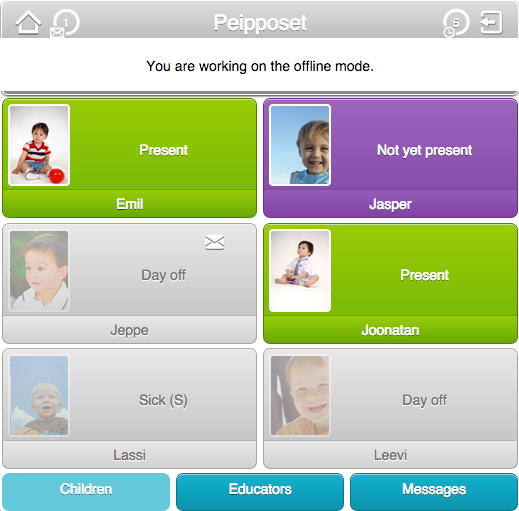
\includegraphics[width=0.6\textwidth]{assets/offline-ui.png}
\end{center}
\caption{Kindergarten UI's care group view, offline mode being active. The size of the presence marking queue is indicated at the top right corner of the user interface.}
\label{fig:offline-ui}
\end{figure}


When the user creates a new Presence Marking on the Kindergarten UI (for example logs child in to the kindergarten when he/she arrives), a new Promise is created which includes Ajax request to the backend. Request's payload is the new Presence Marking. That Promise is then added to the job queue. In Figure~\ref{fig:offline-ui} a screenshot of the Kindergarten UI is given while the offline mode is active. In the figure, the size of the job queue is indicated to be \textit{five}.

While the Online mode is active, job queue constantly looks for the oldest job on the queue and tries to execute it. Executing it means activating the Ajax request inside the Promise. After the request is successfully sent to the backend and a response is received, the promise marks itself as \textit{solved} and that job is then removed from the queue. This process is repeated within a configured interval as long as the application is active on user's browser. If an ongoing request fails due to a network error, the application fall backs to the Offline mode, and the job queue execution halts until Internet connectivity is gained again. It is possible for the request also to fail due a mismatched parameters, which causes the job being removed from the queue.

The state of the queue is saved on the local storage to address the case where the user shuts down the application before the whole queue is sent to the server. Therefore every time the application starts the queue is initialized from the contents stored locally on the user's browser. However also this solution outsources some of the responsibility to the user: in order to have up-to-date information about the attendance status every nurse must ensure that the queue is empty when their shift ends.  % HOX onko näin oikeasti? HOX IMPR pitäisikö viimeisen lauseen juttu siirtää evaluation -kappaleeseen?









%% ###
\subsection{Storing and Receiving Presence Markings on the Backend}
\label{subsec:backend-implementation}
% "Storing and Receiving Presence Markings on the Backend"
% - ainoa offlineen liittyvä muutos mikä toteutettiin bäkkäriin
% - presenceille timestamp, milloin ne on tehty -> voi (ja on) eri kuin mitä vastaanottotimestamp on
% -> yliyksinkertaistaen käytännössä kaikista merkinnöistä tuli "offlinessä-tehtyjä" verrattuna aikaisempaan, missä merkintöihin otettiin timestampit serverille saapumisajan mukaan
% - Tänne jotain juttua kellosynkasta pingauksen yhteydessä? Vai pitäisikö siitä taruilla ton network-laatutunnistuksen yhteydessä?

Due to the simplicity of the offline support required for Päikky, most of the code related work was done on the Kindergarten UI only. Only offline supported feature which needed modifications to the backend was the ability for the user to create Presence Markings without active Internet connection at the time. This required some changes to be done on the mechanisms which receives and stores the Presence Markings coming from the Kindergarten UI. 

Before the offline support Kindergarten UI did not send timestamps of the created Presence Markings to the backend. Timestamps were created on the backend at the time when the requests from the Kindergarten UI were received. 

To allow the postponed sending of the Presence Markings created in the past, the responsibility of creating the timestamps for the markings had to be moved from the backend to the Kindergarten UI. Since the client's clock can be set to anything, this created a need for a mechanism that could synchronize the clocks between the backend and the application.

Since the precision required by the application area is closer to a minute than a second, the client-backend clock synchronization could be done with a quite simple and straightforward approach. The same ping functionality which is used to determine the network status has also the ability to measure the time spent from sending the request from the client to the receiving of the backend's response. When this interval is known, the offset of the clocks on the application and on the backend can be determined. The backend returns the timestamp when the ping request is received on the backend to the application. When the measured duration of the request is split into half, the application can determine what is the offset between its and the backend's clocks. This offset is saved to the local storage, and added to each presence markings timestamp. 

% hox tänne tarvittaessa saisi Kimmon tekemän kaavion https://github.com/futurice/mukavait-paivahoito-kindergarten-ui/blob/development/src/js/networkStatus.js

Due to the nature of TCP protocol (on which HTTP packets are delivered), the exact amount of  spent on receiving the response from server can not be measured. Due to handshakes and other required precautions TCP does, more time is spent on the sending and delivering of the request than what it takes the response to arrive from the backend to the application. This creates the basic problem why the clock synchronizing can never be exact with this method. Päikky is configured to allow synchronizing result only from pings done within a three second timeframe, and as stated above, this is easily within the required precision for this use case. For applications where precise clock synchronization would be required, usage of a more sophisticated protocol engineered specially for that purpose would be required. Protocol of choice for that kind of use case could be the \textit{Network Time Protocol (NTP)} \cite{mills_internet_1991}. % <meta: pitäisikö tästä taruilla lisää, vai liekkö tarve? entä tarvitsisiko tänne jotain lähdettä? tännehän saa vertailua NTP:n ja UDP:n käyttöön jos haluaa>






%% ###
\subsection{Duplicating the Presence State Machine}

% (tarviikohan tämän välttämättä olla oma otsikkonsa?)
Before the offline support the backend also validated the state transfer for the Kindergarten UI. If the new Presence type requested by the application was invalid, the backend would have returned a legal state, which the Kindergarten UI would have applied to the current person. From the user experience point of view this could be seen as a slight lag on the changing of the person's state when the new Presence marking was created. Kindergarten UI at time would not have known what the new state would be and therefore was forced to wait for the backend's response. 

%Since there is always a restricted amount of legal presence state transfers, allowing the Kindergarten UI to set the timestamps for the Presence Markings required it to know about the allowed state transitions from a presence status into another. 

In order to enable the Kindergarten UI to know the allowed possible state transfers and to determine the new Presence state. This resulted as a need for duplicating the Presence State Machine from the backend to the Kindergarten UI. Duplicating it created some redundancy to the backend and Kindergarten UI codebases. Having the Presence state machine on both components of Päikky was inevitable, since as the keeper of the master data, removing the state validating from the backend would be shortsighted. Requests made to the API can be tampered with, and the actual payload has to be always validated by the backend. However having the same validation in two places creates a challenge for the developers: both have to be kept in sync in order for the system to operate properly. 

On the positive side, the lag in the user interface with the Presence state transfer got minimized with the added functionality, since new state could be determined on the browser instantly without having to wait for the backend interaction's result.




















